% !TeX program = pdflatex
% Source: dathuynh1108/OCC at 91223d63adc3289786bbdeff16d5feeb59aeb3d7.
% Measured author-source rerun; reduced epochs explicitly selected by the user.
\documentclass[aspectratio=169,professionalfonts,10pt]{beamer}
\usetheme{Boadilla}
\usecolortheme{default}
\setbeamertemplate{navigation symbols}{}
\usepackage[utf8]{inputenc}
\usepackage[T1]{fontenc}
\usepackage{lmodern}
\usepackage{amsmath,amssymb,amsfonts,mathtools,bm}
\usepackage{booktabs,array,tabularx,ragged2e}
\usepackage{graphicx,xcolor,tikz,etoolbox}
\usetikzlibrary{positioning,arrows.meta,calc}
\usepackage{hyperref}
\graphicspath{{assets/}}
\definecolor{navy}{RGB}{16,44,84}
\definecolor{teal}{RGB}{0,122,122}
\definecolor{orange}{RGB}{168,95,18}
\definecolor{softblue}{RGB}{233,240,250}
\definecolor{softgreen}{RGB}{232,244,239}
\definecolor{softorange}{RGB}{252,239,226}
\definecolor{softgray}{RGB}{245,245,245}
\setbeamercolor{title}{fg=navy}
\setbeamercolor{frametitle}{fg=navy,bg=navy!6}
\setbeamercolor{structure}{fg=navy}
\setbeamercolor{normal text}{fg=black,bg=white}
\setbeamercolor{block title}{fg=white,bg=navy}
\setbeamercolor{block body}{fg=black,bg=navy!5}
\setbeamercolor{block title alerted}{fg=orange,bg=softorange}
\setbeamercolor{block body alerted}{fg=black,bg=softorange!55}
\setbeamercolor{alerted text}{fg=orange}
\setbeamertemplate{blocks}[rounded][shadow=false]
\setbeamerfont{title}{series=\bfseries,size=\LARGE}
\setbeamerfont{frametitle}{series=\bfseries,size=\large}
\setbeamerfont{block title}{series=\bfseries,size=\normalsize}
\setbeamersize{text margin left=0.62cm,text margin right=0.62cm}
\def\phase{OCC REPRODUCTION}
\setbeamertemplate{footline}{%
\leavevmode\hbox to \paperwidth{\hspace{0.62cm}{\scriptsize\color{navy!65}\phase}\hfill
{\scriptsize\color{navy}\insertframenumber\,/\,\inserttotalframenumber}\hspace{0.6cm}}\vspace{0.13cm}}
\newcommand{\RR}{\mathbb R}
\newcommand{\MM}{\mathcal M}
\newcommand{\Cand}{\mathcal C}
\newcommand{\TT}{\mathcal T}
\newcommand{\norm}[1]{\left\lVert#1\right\rVert}
\newcommand{\head}[1]{\par{\normalsize\bfseries\color{navy}#1}\par\vspace{2pt}}
\newcommand{\remarktext}[1]{\par\smallskip{\footnotesize\color{navy!85}#1}\par}
\newcommand{\src}[1]{\par\smallskip{\scriptsize\color{navy!65}#1}\par}
\newcommand{\band}[1]{\begin{beamercolorbox}[rounded=true,sep=0.17cm]{block body}#1\end{beamercolorbox}}
\newcommand{\tightmath}{\setlength{\abovedisplayskip}{4pt}\setlength{\belowdisplayskip}{4pt}\setlength{\abovedisplayshortskip}{2pt}\setlength{\belowdisplayshortskip}{2pt}}
\appto\normalsize{\tightmath}\appto\small{\tightmath}\appto\footnotesize{\tightmath}
\newcolumntype{Y}{>{\RaggedRight\arraybackslash}X}
\title{Normality Bubble Diffusion}
\subtitle{Source-audited methods and shared MVTec results}
\author{Huynh Thanh Dat}
\date{September 2026}
\hypersetup{pdftitle={Normality Bubble Diffusion},pdfauthor={Huynh Thanh Dat},pdfsubject={Source-audited native methods and common MVTec; reduced epoch budgets}}

\newcommand{\resultsrc}[1]{\src{\href{https://github.com/dathuynh1108/OCC/tree/91223d63adc3289786bbdeff16d5feeb59aeb3d7/results/mvtec-full-v2}{OCC / mvtec-full-v2 @ 91223d6} \;|\; #1}}

\begin{document}
\begin{frame}[plain]
\vspace{0.20cm}
\begin{center}
\begin{beamercolorbox}[wd=0.94\paperwidth,rounded=true,sep=0.38cm,center]{block title}
{\usebeamerfont{title}\color{white}Normality Bubble Diffusion}\\[0.3em]
{\large\color{white}Source-audited methods and shared MVTec results}
\end{beamercolorbox}
\vspace{0.18cm}
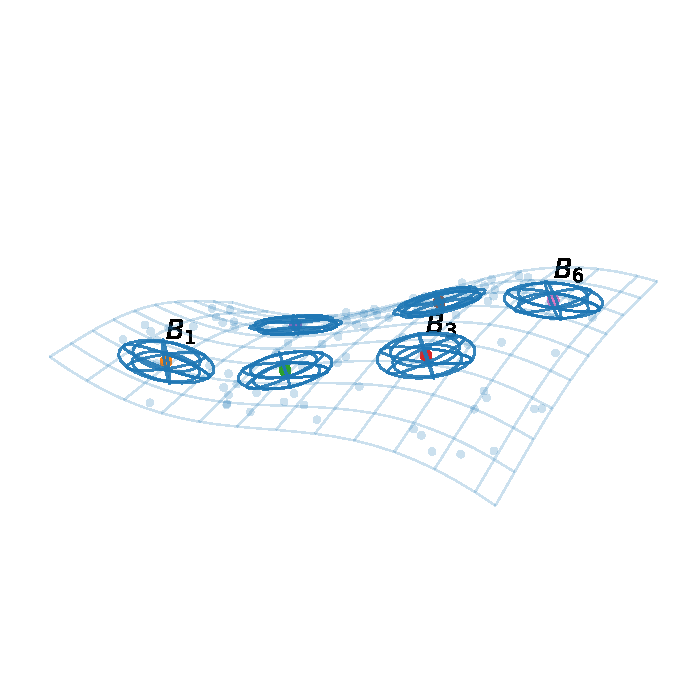
\includegraphics[width=10.1cm,height=3.5cm,keepaspectratio]{manifold3d.pdf}
\par\vspace{0.06cm}
{\large\textbf{Huynh Thanh Dat}}\quad{\normalsize 14 September 2026}
\vspace{0.28cm}
\par{\small Native methods $\;\to\;$ Shared MVTec $\;\to\;$ NBD}
\end{center}
\end{frame}
\begin{frame}[t]{One-class detection}
\vspace{0.23cm}
\begin{columns}[T,onlytextwidth]
\column{.40\textwidth}
\head{Train on normal data}
\[
\mathcal D_N=\{x_i\}_{i=1}^{n}.
\]
\vspace{0.15cm}
\head{Score new observations}
\[
s(x):\mathcal X\to\RR.
\]
A larger score means more anomalous.
\vspace{0.30cm}
\band{Common MVTec train/calibration: normal only.\\[0.1cm]Test: normal + anomaly.}
\column{.56\textwidth}
\centering
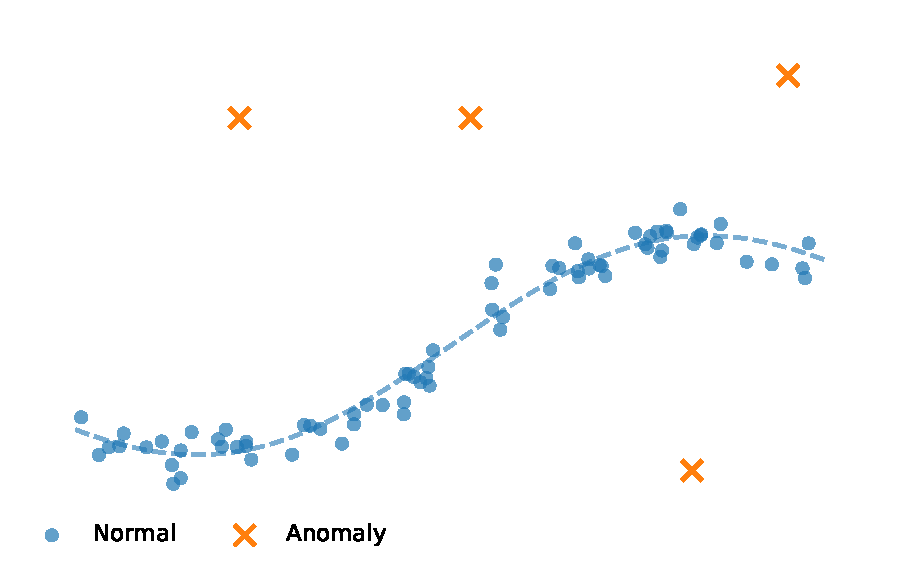
\includegraphics[width=\linewidth,height=4.8cm,keepaspectratio]{problem.pdf}
\src{Schematic: normal support can be curved.}
\end{columns}
\vspace{0.28cm}
\remarktext{Common MVTec uses shared frozen CNN descriptors. Native methods use their own input pipelines.}
\end{frame}

\begin{frame}[t]{Two evaluation tracks}
\small
\begin{center}
\renewcommand{\arraystretch}{1.16}
\begin{tabular}{lrr}
\toprule
\textbf{Track} & \textbf{Data} & \textbf{Purpose} \\
\midrule
Native methods & MNIST / CIFAR / MVTec & Method-specific replication \\
Common benchmark & MVTec:15 categories & Same features and splits \\
\bottomrule
\end{tabular}
\end{center}

\begin{itemize}
\item User-selected runtime budget: about two hours; training epochs shortened.
\item Keep all selected classes, categories and seeds in the coverage manifest.
\item Native image CNNs and shared-feature heads are different experiments.
\end{itemize}

\vfill
\band{\small Full data does not mean full paper training schedule.}

\end{frame}

\begin{frame}[t]{PatchCore: author feature extractor}
\small
\remarktext{Author Quick Guide: ImageNet-pretrained WRN-50 / 224 input / 1,024-D / 10\% coreset.}
\vspace{.12cm}
\begin{center}
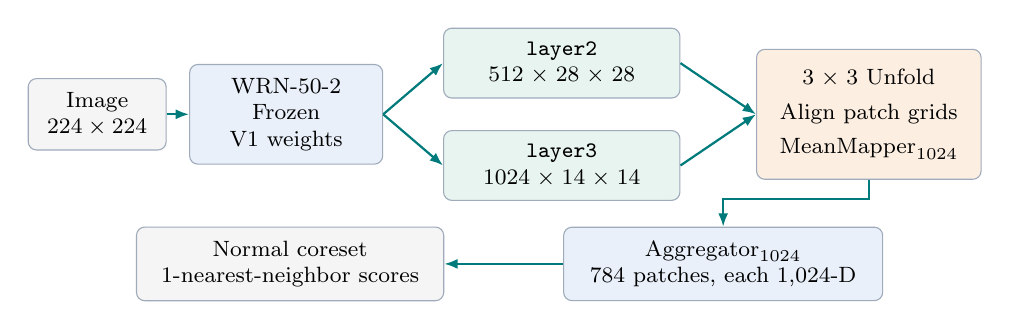
\begin{tikzpicture}[
 box/.style={rounded corners=3pt,draw=navy!40,minimum height=.88cm,align=center,inner sep=5pt,font=\footnotesize},
 arr/.style={-{Latex[length=1.7mm]},thick,draw=teal}]
\node[box,fill=softgray,text width=1.40cm] (im) at (0,0) {Image\\$224\times224$};
\node[box,fill=softblue,text width=2.10cm] (cnn) at (2.4,0) {WRN-50-2\\Frozen\\V1 weights};
\node[box,fill=softgreen,text width=2.65cm] (l2) at (5.9,.65) {\texttt{layer2}\\$512\times28\times28$};
\node[box,fill=softgreen,text width=2.65cm] (l3) at (5.9,-.65) {\texttt{layer3}\\$1024\times14\times14$};
\node[box,fill=softorange,text width=2.50cm,minimum height=1.65cm] (patch) at (9.8,0) {$3\times3$ Unfold\\\smallskip Align patch grids\\\smallskip $\operatorname{MeanMapper}_{1024}$};
\draw[arr](im)--(cnn);\draw[arr](cnn.east)--(l2.west);\draw[arr](cnn.east)--(l3.west);
\draw[arr](l2.east)--(patch.west);\draw[arr](l3.east)--(patch.west);
\node[box,fill=softblue,text width=3.7cm] (agg) at (7.95,-1.90) {$\operatorname{Aggregator}_{1024}$\\784 patches, each 1,024-D};
\node[box,fill=softgray,text width=3.55cm] (mem) at (2.45,-1.90) {Normal coreset\\1-nearest-neighbor scores};
\draw[arr](patch.south)--++(0,-.24)-|(agg.north);\draw[arr](agg.west)--(mem.east);
\end{tikzpicture}
\end{center}
\vspace{-.10cm}
\band{\footnotesize Current rerun: author 1,024-D descriptors. Preserve the startup BN shape probe, then freeze/eval. Native image maximum; common table top-1\% mean.}
\src{Paper Eq. (7): extra neighbor reweighting. Inspected author code: maximum patch score. Separate targets.}
\src{\href{https://github.com/amazon-science/patchcore-inspection/blob/fcaa92f124fb1ad74a7acf56726decd4b27cbcad/src/patchcore/patchcore.py}{\textcolor{teal}{GitHub: patchcore.py}}\quad
\href{https://github.com/amazon-science/patchcore-inspection/blob/fcaa92f124fb1ad74a7acf56726decd4b27cbcad/src/patchcore/common.py}{\textcolor{teal}{common.py}}\quad
\href{https://github.com/amazon-science/patchcore-inspection/blob/fcaa92f124fb1ad74a7acf56726decd4b27cbcad/README.md}{\textcolor{teal}{Author run command}}}
\end{frame}

\begin{frame}[t]{PatchCore: native MVTec result}
\small
\begin{center}
\renewcommand{\arraystretch}{1.16}
\begin{tabular}{lrrr}
\toprule
\textbf{Dataset} & \textbf{Variant} & \textbf{Paper (\%)} & \textbf{Measured (\%)} \\
\midrule
mvtec & author code & 99.00 & 99.02 $\pm$ 0.14 \\
\bottomrule
\end{tabular}
\end{center}
\remarktext{Pixel AUROC: 98.11\%. AUPRO not evaluated.}
\begin{itemize}
\item Full normal train; 10\% coreset; 1NN squared L2; image maximum.
\item WR50-2 ImageNet V1; all 15 categories, three seeds.
\item Released author code omits paper Eq.(7) reweighting.
\end{itemize}
\src{Measured rerun: \href{https://github.com/dathuynh1108/OCC/tree/main/results/reproduction-2026-09-14}{OCC / reproduction-2026-09-14}. See CSVs and source audit.}
\end{frame}


\begin{frame}[t]{Deep SVDD: collapse and safeguards}
\small
\[s(x)=\|f_\theta(x)-c\|^2,\qquad f_\theta(x)\equiv c\ \Rightarrow\ s(x)=0.\]
\begin{itemize}
\item Train the image CNN end to end; fix a nonzero center $c$.
\item No convolution/linear bias; non-affine BatchNorm; leaky ReLU.
\item Reconstruct normal images with an AE, copy its encoder, discard the decoder.
\item AE is an initialization; output variance is a collapse diagnostic.
\end{itemize}

\vfill
\band{\small MNIST: conv 8/4 $\to$32. CIFAR: conv 32/64/128 $\to$128. No ImageNet backbone.}
\src{\href{https://github.com/lukasruff/Deep-SVDD/tree/e20f18c8d0ad9dc01cad09fdf311bd861351a9ad}{Original Theano source} $\mid$ \href{https://github.com/lukasruff/Deep-SVDD-PyTorch/tree/1901612d595e23675fb75c4ebb563dd0ffebc21e}{Executed author PyTorch modules}.}
\end{frame}


\begin{frame}[t]{Deep SVDD: native image CNNs}
\small
\begin{center}
\renewcommand{\arraystretch}{1.16}
\begin{tabular}{lrrr}
\toprule
\textbf{Dataset} & \textbf{Variant} & \textbf{Paper (\%)} & \textbf{Measured (\%)} \\
\midrule
cifar10 & one-class & 64.81 & 61.09 $\pm$ 0.62 \\
cifar10 & soft boundary & 63.28 & 61.52 $\pm$ 0.63 \\
mnist & one-class & 94.80 & 92.69 $\pm$ 0.74 \\
mnist & soft boundary & 93.53 & 92.73 $\pm$ 0.78 \\
\bottomrule
\end{tabular}
\end{center}

\begin{itemize}
\item Author PyTorch LeNet modules; AE 5 + SVDD 12 epochs.
\item Soft-boundary warmup 10; final epoch; 10 classes $\times$10 seeds.
\item Later author-code replication; original Theano numeric parity unverified.
\end{itemize}
\src{Paper: \href{https://proceedings.mlr.press/v80/ruff18a/ruff18a.pdf}{Ruff et al., Table 1}; class macro of printed means. Protocols differ.}\src{Measured rerun: \href{https://github.com/dathuynh1108/OCC/tree/main/results/reproduction-2026-09-14}{OCC / reproduction-2026-09-14}. See CSVs and source audit.}
\end{frame}


\begin{frame}[t]{DROCC: how negatives are generated}
\small
\begin{columns}[T]\begin{column}{.48\textwidth}
\centering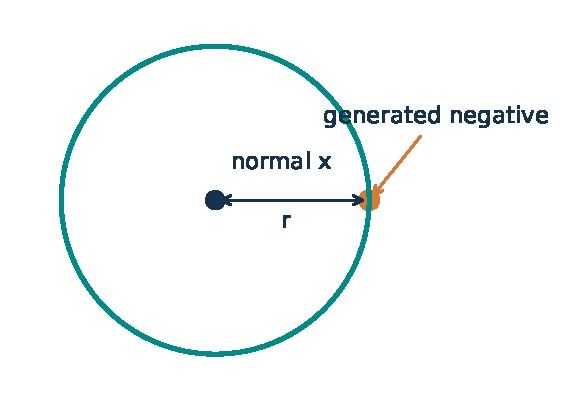
\includegraphics[width=.98\textwidth,height=3.5cm,keepaspectratio]{drocc_source_sampling.pdf}
\end{column}\begin{column}{.49\textwidth}
\begin{itemize}
\item Add Gaussian noise to a normal image.
\item Ascend the loss for the anomaly target.
\item Project displacement to $[r,\gamma r]$.
\item Train on the resulting negative.
\end{itemize}
\end{column}\end{columns}
\vfill
\band{\small CIFAR author code: 50 ascent steps; project every 10; $\gamma=1$ gives a sphere.}
\src{\href{https://github.com/microsoft/EdgeML/tree/81025fce8ba28707eabe72e11bf3987a8d745608/examples/pytorch/DROCC}{Author CIFAR runner} $\mid$ \href{https://github.com/microsoft/EdgeML/blob/81025fce8ba28707eabe72e11bf3987a8d745608/pytorch/edgeml_pytorch/trainer/drocc_trainer.py}{Adversarial training source}.}
\end{frame}


\begin{frame}[t]{DROCC: native CIFAR result}
\small
\begin{center}
\renewcommand{\arraystretch}{1.16}
\begin{tabular}{lrrr}
\toprule
\textbf{Dataset} & \textbf{Variant} & \textbf{Paper (\%)} & \textbf{Measured (\%)} \\
\midrule
cifar10 & fixed final & 74.23 & 64.71 $\pm$ 2.18 \\
cifar10 & best test epoch & 74.23 & 65.99 $\pm$ 2.00 \\
\bottomrule
\end{tabular}
\end{center}

\begin{itemize}
\item Author image CNN and Table 11 parameters; five epochs.
\item All 10 classes, three seeds; 5,000 train normals / 10,000 test.
\item Best-test epoch uses test labels; interpret it as optimistic.
\end{itemize}
\src{Paper: \href{https://proceedings.mlr.press/v119/goyal20c/goyal20c.pdf}{Goyal et al., Table 1}; class macro of printed means. Protocols differ.}\src{Measured rerun: \href{https://github.com/dathuynh1108/OCC/tree/main/results/reproduction-2026-09-14}{OCC / reproduction-2026-09-14}. See CSVs and source audit.}
\end{frame}


\begin{frame}[t]{Kernel SVDD: source protocol and limits}
\small
\begin{center}
\renewcommand{\arraystretch}{1.16}
\begin{tabular}{lrrr}
\toprule
\textbf{Dataset} & \textbf{Variant} & \textbf{Paper (\%)} & \textbf{Measured (\%)} \\
\midrule
cifar10 & $\nu=.01$ & 64.78 & 60.56 $\pm$ 0.20 \\
cifar10 & $\nu=.1$ & 64.78 & 60.67 $\pm$ 0.26 \\
mnist & $\nu=.01$ & 91.29 & 95.51 $\pm$ 0.05 \\
mnist & $\nu=.1$ & 91.29 & 95.51 $\pm$ 0.04 \\
\bottomrule
\end{tabular}
\end{center}

\begin{itemize}
\item Ruff image baseline: train-only PCA 95\%, full kernel fit.
\item Gamma tuned on 1,000 labeled test images; evaluate the other 9,000.
\item Modern libsvm / Gaussian SVDD equivalence checked by independent QP.
\end{itemize}

\vfill
\band{\small Tax--Duin2004 original numeric table remains unreproduced: missing exact folds and search settings.}
\src{\href{https://github.com/DMJTax/dd_tools/tree/efaaf04efae1f8be78906836a5d31547b48be7af}{Tax author reference toolbox} $\mid$ Paper column: \href{https://proceedings.mlr.press/v80/ruff18a/ruff18a.pdf}{Ruff Table 1, better nu}; measured: 10 seeds per nu.}
\end{frame}


\begin{frame}[t]{Common MVTec: one shared benchmark}
\small
\begin{center}
\renewcommand{\arraystretch}{1.16}
\begin{tabular}{lrr}
\toprule
\textbf{Normal train} & \textbf{Test normal} & \textbf{Test anomaly} \\
\midrule
3,629 & 467 & 1,258 \\
\bottomrule
\end{tabular}
\end{center}

\begin{itemize}
\item 15 categories $\times$3 seeds; author WR50/V1 1,024-D descriptors.
\item Image split:60\% FIT /20\% component calibration /remainder threshold.
\item All methods: top1\% patch mean; normal-only image thresholds.
\item Deep head: AE 5+SVDD 15; DROCC head:15 epochs including10 warmup.
\end{itemize}

\vfill
\band{\small Feature heads are controlled adaptations; the CNN is frozen.}

\end{frame}


\begin{frame}[t]{Common MVTec: baseline results}
\small

\centering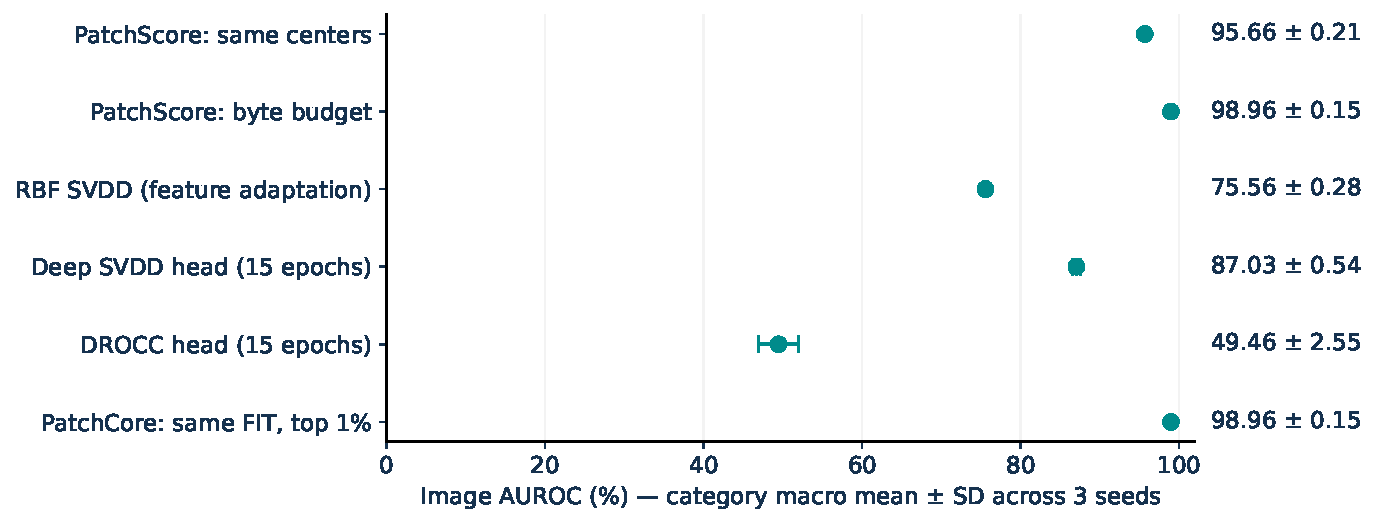
\includegraphics[width=.98\textwidth,height=4.3cm,keepaspectratio]{rerun_baselines.pdf}

\vfill
\band{\small PatchCore keeps a 10\% coreset. PatchScore byte budget is the separate NBD memory control.}
\src{Measured rerun: \href{https://github.com/dathuynh1108/OCC/tree/main/results/reproduction-2026-09-14}{OCC / reproduction-2026-09-14}. See CSVs and source audit.}
\end{frame}


\begin{frame}[t]{Common MVTec: operating points}
\small
\begin{center}
\renewcommand{\arraystretch}{1.16}
\begin{tabular}{lrr}
\toprule
\textbf{Method} & \textbf{FPR (\%)} & \textbf{TPR (\%)} \\
\midrule
PatchScore: same centers & 11.40 & 79.97 \\
PatchScore: byte budget & 13.71 & 89.30 \\
RBF SVDD & 7.27 & 41.69 \\
Deep SVDD head & 4.92 & 58.05 \\
DROCC head & 4.46 & 8.43 \\
PatchCore: same FIT, top 1\% & 13.35 & 89.28 \\
NBD: B+A+D+F & 11.16 & 46.73 \\
\bottomrule
\end{tabular}
\end{center}

\vfill
\band{\small $\alpha=.05$, $k=\lceil(n+1)\cdot.95\rceil$; threshold $=\infty$ if $k>n$; strict $s>\tau$.}
\src{Measured rerun: \href{https://github.com/dathuynh1108/OCC/tree/main/results/reproduction-2026-09-14}{OCC / reproduction-2026-09-14}. See CSVs and source audit.}
\end{frame}

\begin{frame}[t]{NBD: local bubbles, one shared graph}
\vspace{0.13cm}
\begin{columns}[T,onlytextwidth]
\column{.65\textwidth}
\centering
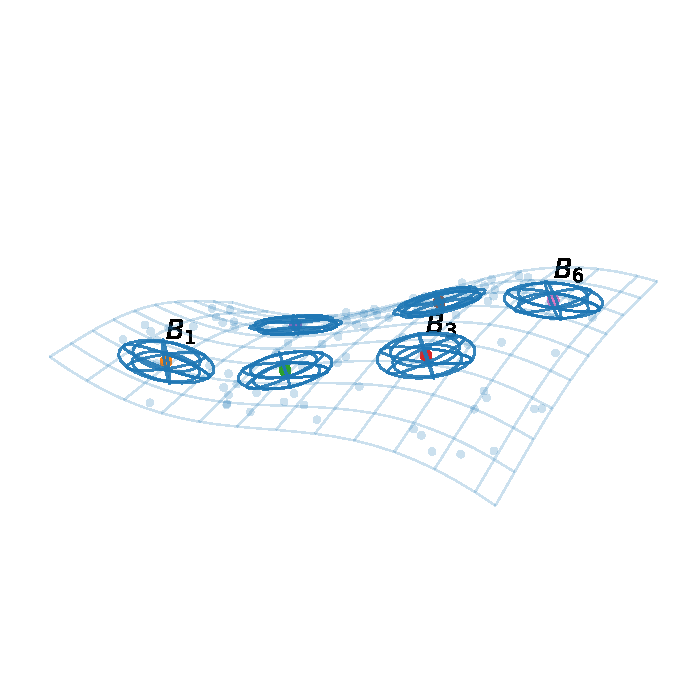
\includegraphics[width=\linewidth,height=4.2cm,keepaspectratio]{manifold3d.pdf}
\src{Schematic: local ellipsoids around a curved surface.}
\column{.31\textwidth}
\head{Each bubble stores}
A center, tangent variation, and normal thickness.
\vspace{0.34cm}
\head{The graph connects them}
Diffusion compares the regions each bubble can reach.
\end{columns}
\vspace{0.28cm}
\band{\centering Normal features $\to$ bubbles $\to$ shared graph $\to$ diffusion distance $\to$ query score}
\remarktext{Hypothesis tested: a normal query has local support and attaches to a coherent region of the graph.}
\end{frame}
\begin{frame}[t]{A local normality bubble}
\small
\[
B_j=(c_j,U_j,\Lambda_j,\sigma_{\perp,j}^2),\qquad
U_j^\top U_j=I_{d_j},\qquad\Pi_j=U_jU_j^\top.
\]
\begin{columns}[T,onlytextwidth]
\column{.57\textwidth}
\head{Local model}
\[
z=c_j+U_ja+\varepsilon_{\perp,j},\qquad a\perp\!\!\!\perp\varepsilon_{\perp,j},
\]
\[
a\sim\mathcal N(0,\Lambda_j),\qquad
\varepsilon_{\perp,j}\sim\mathcal N\!\left(0,\sigma_{\perp,j}^2(I-\Pi_j)\right).
\]
\[
\boxed{\Sigma_j=U_j\Lambda_jU_j^\top+\sigma_{\perp,j}^2(I-\Pi_j).}
\]
\column{.39\textwidth}
\centering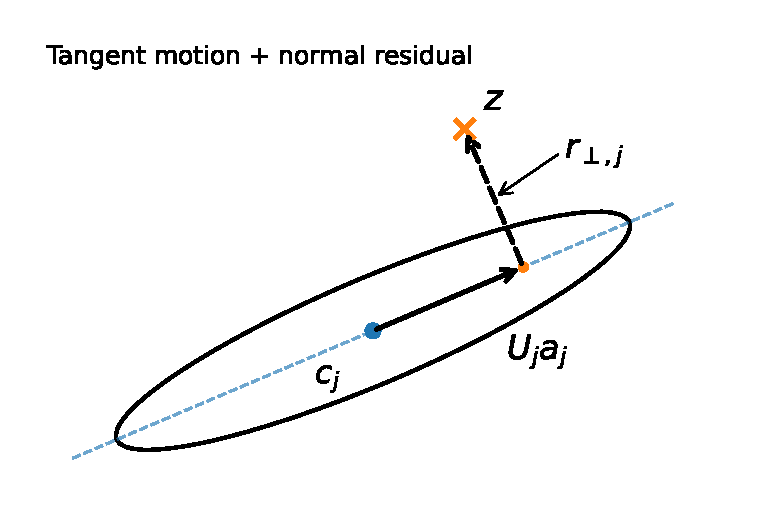
\includegraphics[width=\linewidth,height=2.90cm,keepaspectratio]{bubble_detail.pdf}
\end{columns}
\vspace{0.10cm}
\head{Fit by local PCA}
Neighborhood mean $\to c_j$; top $d_j$ eigenpairs $\to U_j,\Lambda_j$.
\[
\sigma_{\perp,j}^2=\frac1{D-d_j}\sum_{k=d_j+1}^{D}\widehat\lambda_{jk}.
\]
\remarktext{Executed: 128 bubbles; 128 neighbors; $d_j=16$. The same-center control uses the fitted neighborhood means $c_j$.}
\end{frame}
\begin{frame}[t]{Scoring a query}
\small
\[
a_j(z)=U_j^\top(z-c_j),\qquad
r_{\perp,j}(z)=(I-\Pi_j)(z-c_j).
\]
\begin{block}{Local energy}
\[
E_j(z)=
\underbrace{\frac{a_j^\top(\Lambda_j+\epsilon I)^{-1}a_j}{d_j}}_{\text{tangent rarity}}
+\beta\underbrace{\frac{\norm{r_{\perp,j}}_2^2}{(D-d_j)(\sigma_{\perp,j}^2+\epsilon)}}_{\text{off-manifold residual}}.
\]
\end{block}
\vspace{0.02cm}
\begin{columns}[T,onlytextwidth]
\column{.48\textwidth}
\head{Absolute fit}
\[
S_B(z)=\min_{j\in\Cand(z)}E_j(z),
\]
\[
S_A(z)=-T_b\log\!\left[\frac1K\sum_{j\in\Cand(z)}e^{-E_j(z)/T_b}\right].
\]
\column{.48\textwidth}
\head{Attachment to the graph}
\[
b_j(z)=\frac{e^{-E_j(z)/T_b}}{\sum_{k\in\Cand(z)}e^{-E_k(z)/T_b}}.
\]
\remarktext{$K=|\Cand(z)|$ candidates; $b_j=0$ outside.\\$\sum_jb_j(z)=1$.}
\end{columns}
\src{Executed: $K=8$, $T_b=1$, $\beta=1$, $\epsilon=10^{-6}$. This dimension-normalized energy is not Gaussian NLL.}
\end{frame}
\begin{frame}[t]{Comparing two bubbles}
\small
\vspace{0.08cm}
\begin{columns}[T,onlytextwidth]
\column{.322\textwidth}
\head{Center displacement}
\centering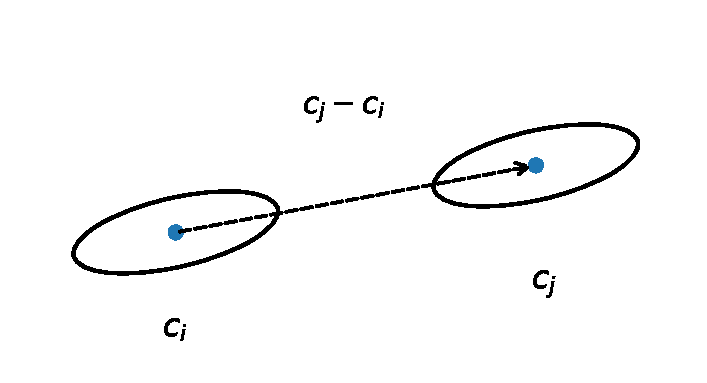
\includegraphics[width=\linewidth,height=1.68cm,keepaspectratio]{pair_centers.pdf}\par\raggedright
\remarktext{Earlier: Euclidean distance}
\[
r_c^{\rm E}(i,j)=\norm{c_i-c_j}_2^2.
\]
\remarktext{Used here: two-way bubble energy}
\[
r_c^{\rm G}(i,j)=\tfrac12\big[E_i(c_j)+E_j(c_i)\big].
\]
\column{.322\textwidth}
\head{Frame disagreement}
\centering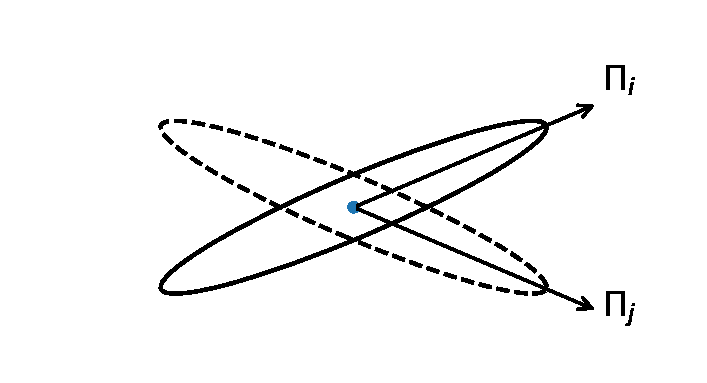
\includegraphics[width=\linewidth,height=1.68cm,keepaspectratio]{pair_frames.pdf}\par\raggedright
\[
r_F(i,j)=\norm{\Pi_i-\Pi_j}_F^2
\]
\[
=d_i+d_j-2\norm{U_i^\top U_j}_F^2.
\]
\remarktext{Compare tangent subspaces, not basis-vector signs.}
\column{.322\textwidth}
\head{Optional: thickness}
\centering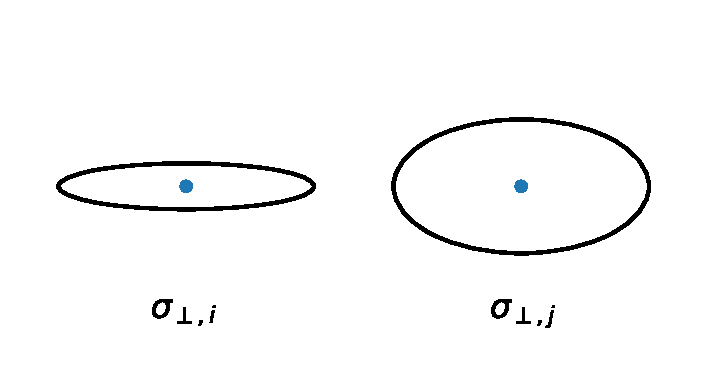
\includegraphics[width=\linewidth,height=1.68cm,keepaspectratio]{pair_thickness.pdf}\par\raggedright
\[
r_\sigma(i,j)=\left[\log\frac{\sigma_{\perp,i}^2+\epsilon}{\sigma_{\perp,j}^2+\epsilon}\right]^2.
\]
\remarktext{Not used in the reported benchmark. Not a full covariance distance.}
\end{columns}
\vspace{0.34cm}
\band{\textbf{Executed graph:} two-way center energy + frame disagreement. Thickness weight is zero.}
\src{The earlier Euclidean distance and the optional thickness term are shown for context, not as tested ablations.}
\end{frame}
\begin{frame}[t]{From bubbles to a graph}
\small
\begin{block}{Edge dissimilarity, before diffusion}
\[
\delta_B(i,j)=\frac{r_c(i,j)}{\tau_c}
+\lambda_F\frac{r_F(i,j)}{\tau_F}.
\]
\end{block}
\begin{columns}[T,onlytextwidth]
\column{.49\textwidth}
\centering\vspace{.20cm}
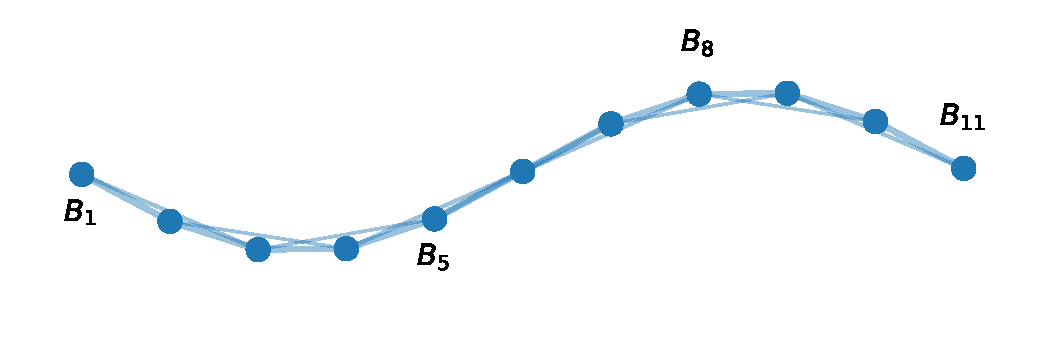
\includegraphics[width=\linewidth,height=2.85cm,keepaspectratio]{bubble_graph.pdf}
\src{Toy graph. Each node is one bubble; thicker edges have larger affinity.}
\column{.47\textwidth}
\head{Affinity and transition}
For symmetric local candidate edges $\mathcal E$,
\[
W_{ij}=\mathbf1_{\{(i,j)\in\mathcal E\}}e^{-\delta_B(i,j)}\quad(i\ne j),
\]
\[
W_{ii}=\eta>0,\qquad s_i=\sum_jW_{ij},
\]
\[
P_{ij}=\frac{W_{ij}}{s_i},\qquad\pi_i=\frac{s_i}{\sum_m s_m}.
\]
\end{columns}
\vspace{0.18cm}
\band{Fit the graph once on normal data. Every query uses the same bubble nodes.}
\src{Executed: 12 graph neighbors; $\lambda_F=1$, $\eta=1$. No thickness penalty. $\delta_B$ need not be a metric.}
\end{frame}
\begin{frame}[t]{Diffusion distance}
\small
Similar $t$-step transition distributions give a smaller diffusion distance:
\[
\boxed{D_t^2(i,j)=\sum_m\frac{\big[(P^t)_{im}-(P^t)_{jm}\big]^2}{\pi_m}.}
\]
\begin{columns}[T,onlytextwidth]
\column{.44\textwidth}
\centering\vspace{0.12cm}
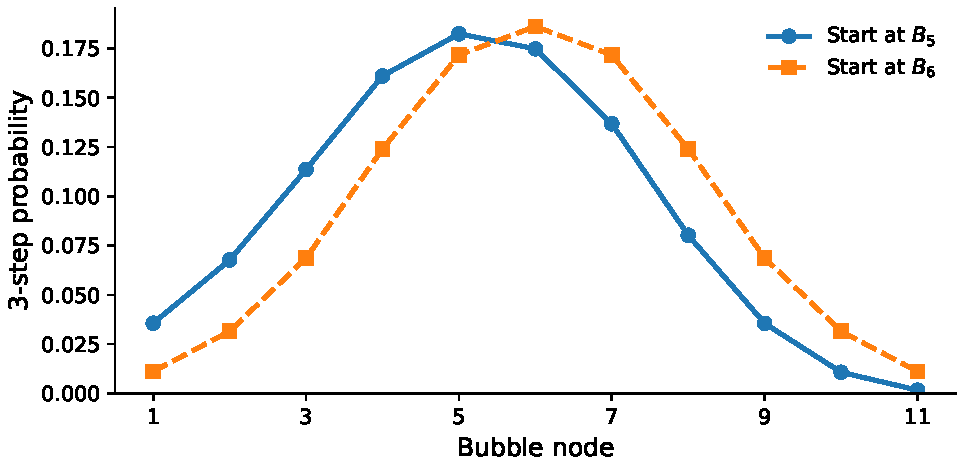
\includegraphics[width=\linewidth,height=2.67cm,keepaspectratio]{diffusion_walks.pdf}
\src{Same toy graph; two neighboring starting nodes, $t=3$.}
\column{.52\textwidth}
\head{Compute with eigenvectors}
\[
P\psi_\ell=\lambda_\ell\psi_\ell,\qquad
\sum_i\pi_i\psi_\ell(i)\psi_k(i)=\delta_{\ell k}.
\]
\[
D_t^2(i,j)=\sum_{\ell=1}^{M-1}\lambda_\ell^{2t}\big[\psi_\ell(i)-\psi_\ell(j)\big]^2.
\]
\[
\Phi_t(B_j)=\big(\lambda_1^t\psi_1(j),\ldots,\lambda_L^t\psi_L(j)\big),
\]
\[
D_{t,L}^2(i,j)=\norm{\Phi_t(B_i)-\Phi_t(B_j)}^2.
\]
\end{columns}
\src{[4] Coifman--Lafon (2006). Executed: all $L=M-1$ nonconstant modes, $\mathcal T=\{1,3,5\}$. The figure is schematic.}
\end{frame}
\begin{frame}[t]{Does the query attach to one region?}
\small
\begin{columns}[T,onlytextwidth]
\column{.48\textwidth}
\centering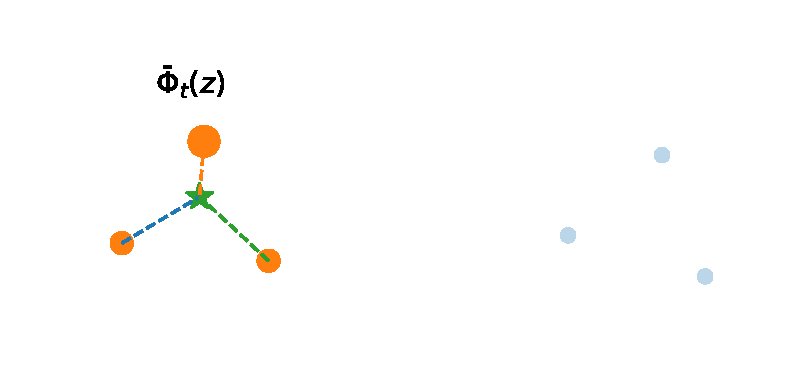
\includegraphics[width=.88\linewidth,height=1.28cm,keepaspectratio]{attachment_near.pdf}
\par\textbf{Nearby bubbles: lower dispersion}
\column{.48\textwidth}
\centering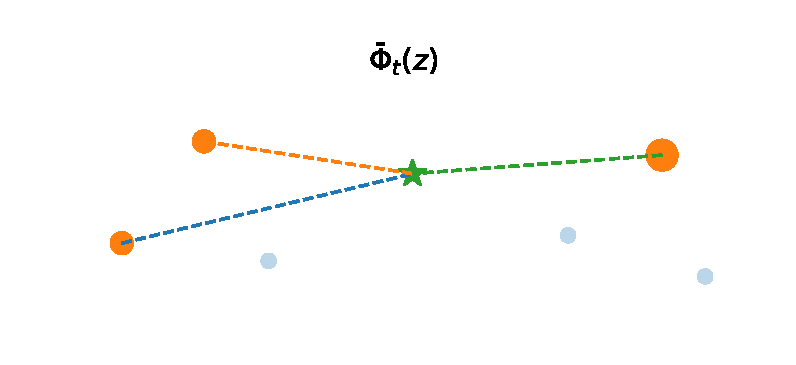
\includegraphics[width=.88\linewidth,height=1.28cm,keepaspectratio]{attachment_far.pdf}
\par\textbf{Distant bubbles: higher dispersion}
\end{columns}
\src{Schematic diffusion coordinates. Circle area: $b_j(z)$. Star: weighted mean.}
\[
\boxed{S_D(z)=\frac1{2|\TT|}\sum_{t\in\TT}\sum_{i,j}b_i(z)b_j(z)D_{t,L}^2(i,j).}
\]
\begin{columns}[T,onlytextwidth]
\column{.50\textwidth}
\head{Equivalent variance at time $t$}
\[
\begin{aligned}
\bar\Phi_t(z)&=\sum_jb_j(z)\Phi_t(B_j),\\[0.2em]
S_{D,t}(z)&=\sum_jb_j(z)\norm{\Phi_t(B_j)-\bar\Phi_t(z)}^2.
\end{aligned}
\]
\column{.46\textwidth}
\head{Frame inconsistency}
\[
S_F(z)=\tfrac12\sum_{i,j}b_i(z)b_j(z)r_F(i,j).
\]
\remarktext{Executed: $\TT=\{1,3,5\}$.}
\end{columns}
\src{A one-bubble outlier can have $S_D\approx0$; $S_B$ and $S_A$ still measure its absolute mismatch.}
\end{frame}
\begin{frame}[t]{NBD: component scaling and final score}
\small
\setlength{\abovedisplayskip}{3pt}\setlength{\belowdisplayskip}{3pt}
\begin{block}{Local fit + diffusion and frame consistency}
\[
\boxed{S_{\rm NBD}(z)=\widetilde S_B(z)+\widetilde S_A(z)+\widetilde S_D(z)+\lambda_F\widetilde S_F(z).}
\]
\end{block}
\textbf{NBD only:} $\mathcal Z_{\rm cal}$ contains patches from the 721 reserved normal images:
\[
\widetilde S_q(z)=-\log\!\left[
\frac{1+\sum_{u\in\mathcal Z_{\rm cal}}\mathbf1_{\{S_q(u)\ge S_q(z)\}}}{|\mathcal Z_{\rm cal}|+1}
\right],\qquad q\in\{B,A,D,F\}.
\]
\vspace{0.02cm}
\begin{center}

\begin{tikzpicture}[box/.style={rounded corners=3pt,minimum height=.60cm,text width=3.9cm,align=center,inner sep=4pt},arr/.style={-{Latex[length=2mm]},thick,draw=teal}]
\node[box,fill=softblue] (z) {Patch features $z_p$};
\node[box,fill=softgreen,right=.40cm of z] (a) {Patch scores $A(x)$};
\node[box,fill=softorange,right=.40cm of a] (s) {Image score};
\draw[arr](z)--(a);\draw[arr](a)--(s);
\end{tikzpicture}
\end{center}
\begin{columns}[T,onlytextwidth]
\column{.43\textwidth}
\[
A(x)_p=S_{\rm NBD}(z_p).
\]
\column{.53\textwidth}
\[
S_{\rm image}(x)=\frac1{|\mathcal P_\rho(x)|}\sum_{p\in\mathcal P_\rho(x)}A(x)_p.
\]
\end{columns}
\src{$\mathcal P_\rho$: top 1\% (8 of 784 patches). $\lambda_F=1$. This is not a calibrated anomaly probability.}
\vspace{0.0cm}
\band{\footnotesize Component scaling uses the reserved subset, not the 734 threshold images.\\[.06cm]
After aggregation, NBD uses the same image-threshold rule as the baselines.}
\end{frame}

\begin{frame}[t]{NBD versus common baselines}
\small

\centering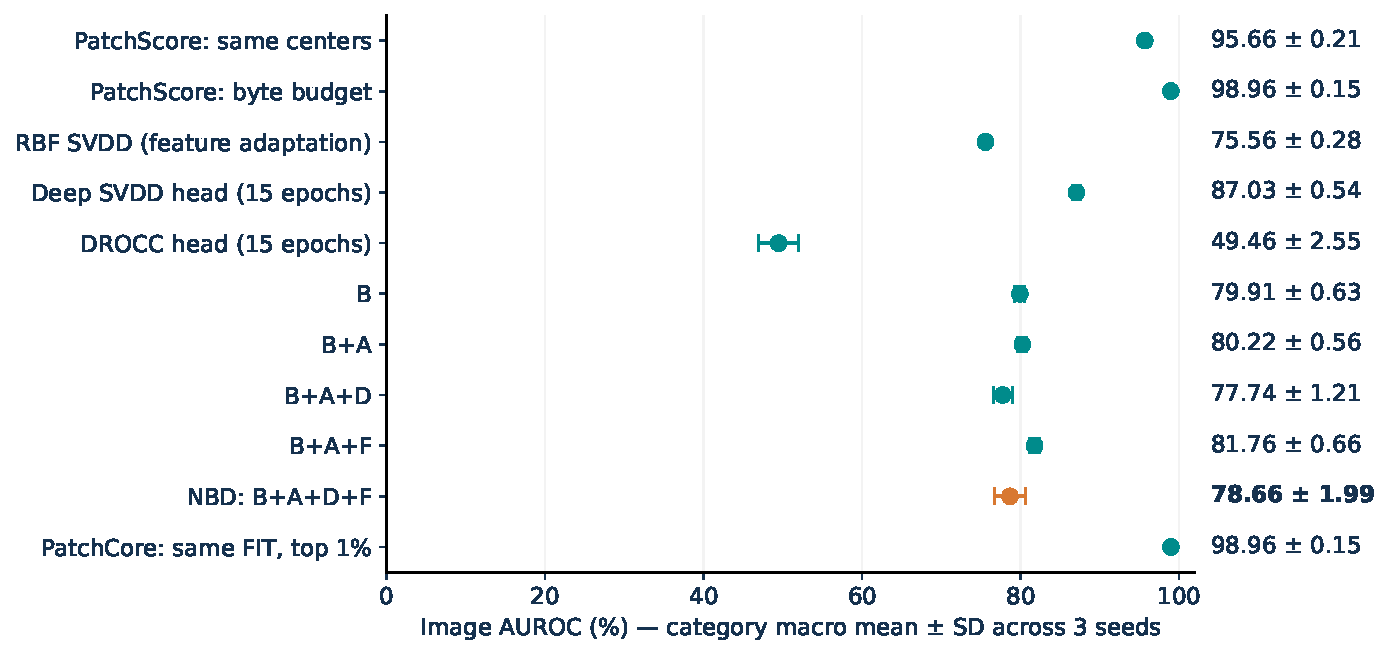
\includegraphics[width=.98\textwidth,height=4.65cm,keepaspectratio]{rerun_all_methods.pdf}
\src{Measured rerun: \href{https://github.com/dathuynh1108/OCC/tree/main/results/reproduction-2026-09-14}{OCC / reproduction-2026-09-14}. See CSVs and source audit.}
\end{frame}


\begin{frame}[t]{Ablations: keep the declared NBD result}
\small

\centering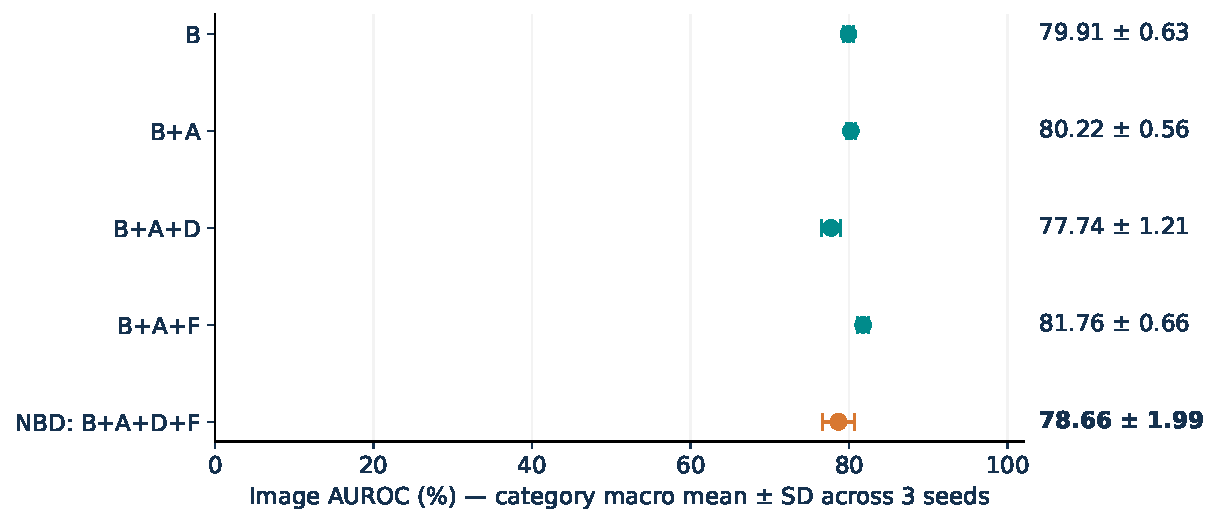
\includegraphics[width=.98\textwidth,height=3.9cm,keepaspectratio]{rerun_ablations.pdf}

\vfill
\band{\small $B$: bubble fit; $A$: support; $D$: diffusion; $F$: frame. Final NBD stays $B+A+D+F$.}
\src{Measured rerun: \href{https://github.com/dathuynh1108/OCC/tree/main/results/reproduction-2026-09-14}{OCC / reproduction-2026-09-14}. See CSVs and source audit.}
\end{frame}


\begin{frame}[t]{All 15 categories, all 11 variants}
\small

\centering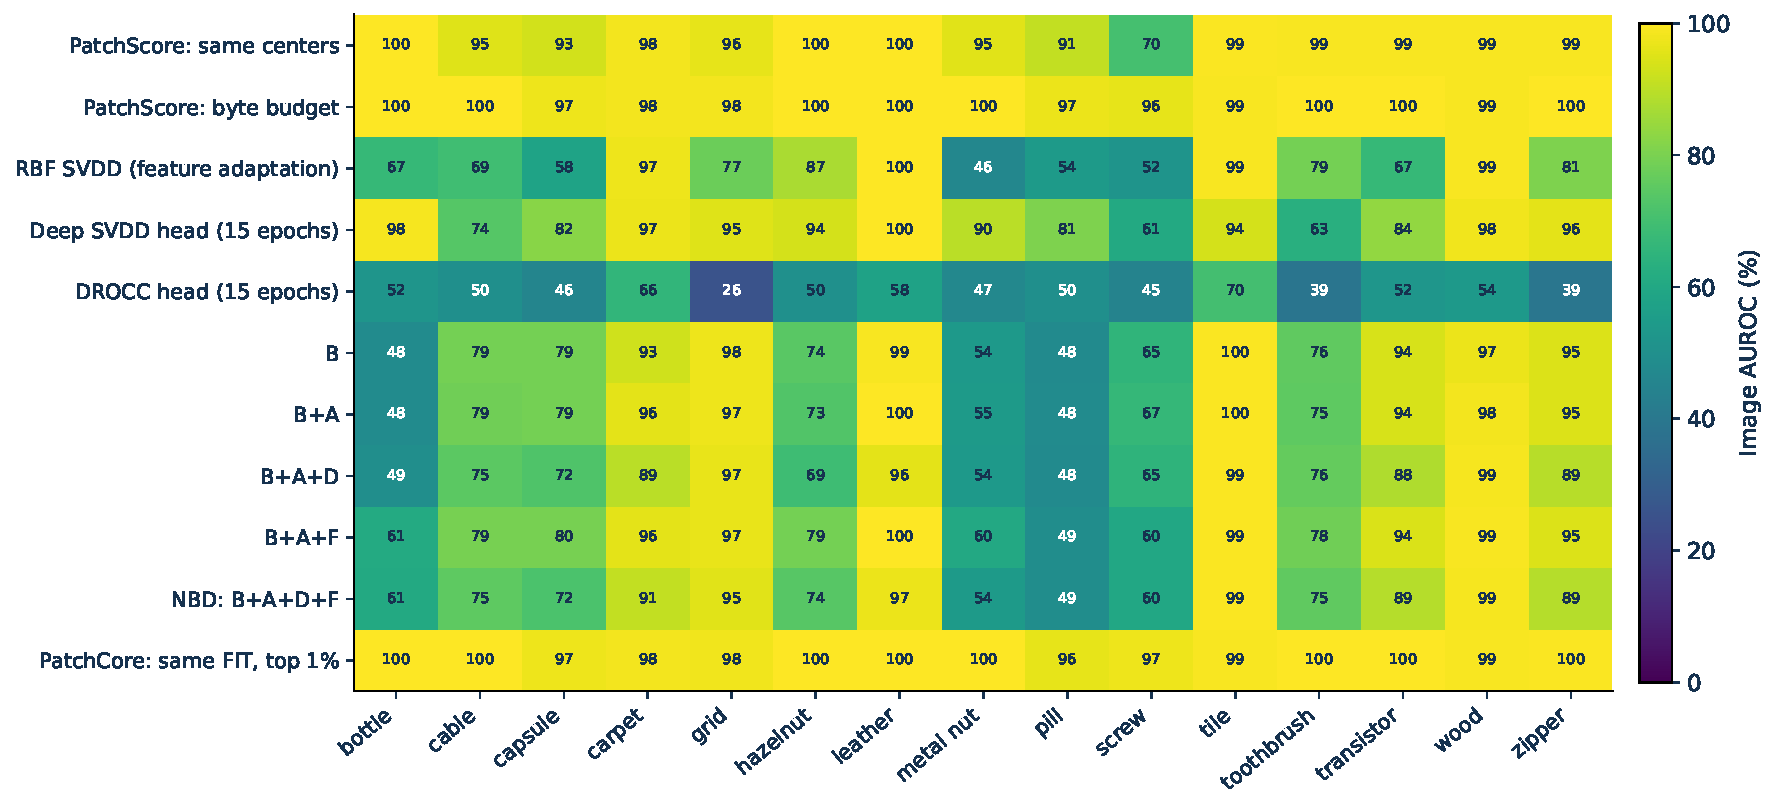
\includegraphics[width=.98\textwidth,height=5.0cm,keepaspectratio]{rerun_categories.pdf}
\src{Measured rerun: \href{https://github.com/dathuynh1108/OCC/tree/main/results/reproduction-2026-09-14}{OCC / reproduction-2026-09-14}. See CSVs and source audit.}
\end{frame}


\begin{frame}[t]{Complete common results}
\small
\footnotesize\begin{center}
\renewcommand{\arraystretch}{1.16}
\begin{tabular}{lrr}
\toprule
\textbf{Method} & \textbf{Image AUROC (\%)} & \textbf{AP (\%)} \\
\midrule
PatchScore: same centers & 95.66 $\pm$ 0.21 & 98.41 $\pm$ 0.10 \\
PatchScore: byte budget & 98.96 $\pm$ 0.15 & 99.70 $\pm$ 0.05 \\
RBF SVDD (feature adaptation) & 75.56 $\pm$ 0.28 & 88.92 $\pm$ 0.19 \\
Deep SVDD head (15 epochs) & 87.03 $\pm$ 0.54 & 94.12 $\pm$ 0.33 \\
DROCC head (15 epochs) & 49.46 $\pm$ 2.55 & 72.88 $\pm$ 1.44 \\
B & 79.91 $\pm$ 0.63 & 91.99 $\pm$ 0.88 \\
B+A & 80.22 $\pm$ 0.56 & 92.20 $\pm$ 0.68 \\
B+A+D & 77.74 $\pm$ 1.21 & 90.65 $\pm$ 0.22 \\
B+A+F & 81.76 $\pm$ 0.66 & 92.75 $\pm$ 0.77 \\
NBD: B+A+D+F & 78.66 $\pm$ 1.99 & 90.99 $\pm$ 0.77 \\
PatchCore: same FIT, top 1\% & 98.96 $\pm$ 0.15 & 99.71 $\pm$ 0.04 \\
\bottomrule
\end{tabular}
\end{center}
\src{Measured rerun: \href{https://github.com/dathuynh1108/OCC/tree/main/results/reproduction-2026-09-14}{OCC / reproduction-2026-09-14}. See CSVs and source audit.}
\end{frame}


\begin{frame}[t]{Coverage and reproducibility}
\small
\begin{center}
\renewcommand{\arraystretch}{1.16}
\begin{tabular}{lr}
\toprule
\textbf{Track} & \textbf{Completed / planned result groups} \\
\midrule
DROCC & 60/60 \\
DeepSVDD & 400/400 \\
Gaussian\_OCSVM\_equiv\_SVDD & 400/400 \\
common\_mvtec & 90/90 \\
native\_patchcore & 45/45 \\
\bottomrule
\end{tabular}
\end{center}

\begin{itemize}
\item Independent image-score audit: 8,262,100 exported predictions.
\item Pinned sources, configs, split IDs, checkpoints, replay and raw CSVs retained.
\item Original full schedules and historical v2 results remain available.
\end{itemize}
\src{Measured rerun: \href{https://github.com/dathuynh1108/OCC/tree/main/results/reproduction-2026-09-14}{OCC / reproduction-2026-09-14}. See CSVs and source audit.}
\end{frame}


\begin{frame}[t]{Inference: shared CNN and scorer costs}
\small
\footnotesize\begin{center}
\renewcommand{\arraystretch}{1.16}
\begin{tabular}{lrr}
\toprule
\textbf{Method} & \textbf{Median ms} & \textbf{State MiB} \\
\midrule
Shared author WR50 descriptor & 30.91 & 263.03 \\
PatchScore: same centers & 1.30 & 0.50 \\
PatchScore: byte budget & 1.47 & 9.01 \\
RBF SVDD & 10.82 & 16.02 \\
Deep SVDD head & 1.41 & 0.25 \\
DROCC head & 1.50 & 0.25 \\
NBD: B+A+D+F & 7.47 & 9.13 \\
PatchCore: same FIT, top 1\% & 1.91 & 38.28 \\
\bottomrule
\end{tabular}
\end{center}

\vfill
\band{\small One bottle image, seed 0; batch 1; 30 repeats. NBD calibration arrays are additional; see report.}
\src{CUDA-synchronized after training. Scorer time excludes shared CNN; state is not peak GPU memory.}
\end{frame}


\begin{frame}[t]{Appendix: historical v2 shared-feature results}
\small
\footnotesize\begin{center}
\renewcommand{\arraystretch}{1.16}
\begin{tabular}{lr}
\toprule
\textbf{Historical method} & \textbf{Image AUROC (\%)} \\
\midrule
PatchScore: same centers & 95.86 $\pm$ 0.23 \\
PatchScore: byte budget & 98.56 $\pm$ 0.21 \\
RBF SVDD (feature adaptation) & 78.20 $\pm$ 0.26 \\
Deep SVDD head (100 epochs) & 81.85 $\pm$ 0.52 \\
DROCC head (100 epochs) & 54.45 $\pm$ 5.43 \\
B & 82.70 $\pm$ 1.81 \\
B+A & 82.80 $\pm$ 1.62 \\
B+A+D & 79.72 $\pm$ 2.46 \\
B+A+F & 82.82 $\pm$ 1.88 \\
NBD: B+A+D+F & 78.79 $\pm$ 2.37 \\
\bottomrule
\end{tabular}
\end{center}

\vfill
\band{\small Previous 1,536-D extractor, AE 50 / heads 100 epochs. Preserved evidence; a different protocol.}
\src{\href{https://github.com/dathuynh1108/OCC/tree/91223d63adc3289786bbdeff16d5feeb59aeb3d7/results/mvtec-full-v2}{Historical v2 at 91223d6}. Do not infer a causal feature effect from this comparison.}
\end{frame}


\begin{frame}[t]{References and evidence}
\small

\begin{itemize}
\item \href{https://proceedings.mlr.press/v80/ruff18a.html}{Ruff et al.: Deep One-Class Classification (2018).}
\item \href{https://proceedings.mlr.press/v119/goyal20c.html}{Goyal et al.: DROCC (2020).}
\item \href{https://github.com/amazon-science/patchcore-inspection}{Roth et al.: PatchCore (2022), released author code.}
\item Tax and Duin: Support Vector Data Description (2004).
\item Coifman and Lafon: Diffusion Maps (2006).
\item \href{https://github.com/dathuynh1108/OCC}{Code, full tables, handoff and source audit: dathuynh1108/OCC.}
\end{itemize}

\vfill
\band{\small Scores describe these declared protocols and training budgets.}

\end{frame}

\end{document}
